\documentclass[12pt]{article}

% 日本語設定
\usepackage{plautopatch}
\usepackage[utf8]{inputenc}
\usepackage{CJKutf8}
\usepackage{otf}

% 必要なパッケージ
\usepackage{amsmath}
\usepackage{amsfonts}
\usepackage{amssymb}
\usepackage[dvipdfmx]{graphicx}
\usepackage{geometry}
\geometry{margin=2.5cm}

\title{情報システム工学演習I レポート\\時系列解析における自己回帰モデルの実践的応用}
\author{学籍番号: 08D23091 \\ 氏名: 辻 孝弥}
\date{\today}

\begin{document}

\maketitle

\section{自己回帰モデル(AR)について}

\subsection{自己回帰モデル(AR)の定義}

自己回帰 (AR) モデルは,「現在の値」を「過去の値」の線形結合として表現する時系列モデルである。次数 $p$ の AR モデル(AR($p$))は次式で定義される。

\[
x_t = c + \sum_{i=1}^{p} \varphi_i\,x_{t-i} + \varepsilon_t
\]

ここで,
\begin{itemize}
\item $x_t$:時点 $t$ の観測値
\item $c$:定数項
\item $\varphi_i$:ラグ $i$ の AR 係数
\item $\varepsilon_t$:平均 0・分散 $\sigma^2$ のホワイトノイズ
\item $p$:モデル次数
\end{itemize}

\subsection{直感的意味}
\begin{itemize}
\item \textbf{自己依存構造}:過去$p$ステップの値が現在値に影響する
\item \textbf{ホワイトノイズ}:モデルが説明できない突発的変動を表現
\item \textbf{定常性条件}:多項式 $1-\varphi_1 z-\dots-\varphi_p z^p=0$ の根が単位円外にあることで長期的な安定性が保証される
\end{itemize}

\subsection{パラメータ推定}
ARモデルのパラメータ推定にはYule–Walker方程式や最尤推定 (MLE) が用いられる。次数選択にはAIC/BICなどの情報量規準が使用される。

\subsection{ACF・PACF の特徴}
ARモデルでは自己相関関数(ACF)は指数的に減衰し,偏自己相関関数(PACF)は次数$p$で切断される特性を持つ。

\subsection{応用例と拡張}
ARモデルは金融リターンの予測や短期需要予測などに広く応用されており,ARMA,ARIMA,VARモデル等への拡張が可能である。

\section{Google Trendsデータの時系列解析}

\subsection{データの考察}

本研究では,Google Trendsから取得した「ワイドパンツ」の検索量データを用いて時系列解析を実施した。

\subsubsection{データの概要}
\begin{itemize}
\item \textbf{検索ワード}:「ワイドパンツ」
\item \textbf{取得期間}:2020年4月19日~2025年4月20日(約5年間,週次データ262点)
\item \textbf{データ範囲}:検索量インデックス 45~100
\item ここで分析対象とするワイドパンツとは,裾幅が広いパンツを指す。
\end{itemize}

\begin{figure}[htbp]
    \centering
    
\includegraphics[width=0.5\textwidth]{./static/22602788.png}
    \caption{ワイドパンツの典型的なデザイン:裾幅が広い}
    \label{fig:wide_pants_design}
\end{figure}

\subsubsection{分析対象の選定理由}
本研究は,単なる演習を超えて,\textbf{実世界のビジネス課題における時系列予測の実用性を探求する}ことを目的としている。\\

ファッション産業における需要予測は,在庫管理,マーケティング戦略,トレンド分析において極めて重要な意思決定支援ツールとなり得る。特にアパレル業界では,季節性と急変するトレンドを正確に予測することが,収益性と競争力を左右する重要な要素となる。\\

本研究において「ワイドパンツ」を分析対象として採用した背景には,時系列解析の実践的学習に適した以下の特性がある。\\

第一に,\textbf{適切なデータ特性}として,検索量インデックスが中程度の範囲(45~100)で変動しており,過度にニッチでも超メジャーでもない適度な検索ボリュームを持つ。これにより,週次データにおいてトレンドと季節性の両方が明確に観察可能である。極端に高い・低い検索頻度のキーワードでは,データが平坦になりすぎるか,ノイズが支配的となり,ARモデルの性能評価が困難となる。

第二に,\textbf{明確な周期性パターン}を有することが挙げられる。ファッション関連キーワードは一般的に季節変動を示すが,ワイドパンツは特に春夏期のカジュアルボトムスとしての需要により,年次周期性が比較的安定している。このような季節性を持つ時系列は,異なるAR次数での予測性能比較において理想的な教材となる。

第三に,\textbf{構造変化を含む現実的なデータ}であることが重要な選定要因である。2024年後半以降のジェンダーレスファッション・リラクシングウェアの流行により,従来の周期パターンを超える急激な検索量増加が観測されている。この特徴により,ARモデルの汎化性能と予測限界を同時に検証することが可能となる。
\\

これらの特性により,\textbf{ワイドパンツは時系列解析における基礎的概念の理解と,実世界データにおけるモデル限界の認識という,両面的な学習効果を提供する最適な研究対象}であると判断した。

\subsubsection{データの特徴}
観測されたデータの主要な特徴は以下の通りである:

\begin{itemize}
\item \textbf{長期トレンド}:全体的に右肩上がりの傾向を示し,ワイドパンツへの関心が時間とともに増加していることが確認された
\item \textbf{季節性}:年次周期性が観察され,特定の季節(春・秋)に検索量が増加する傾向が見られた。これは、春と秋は新作が一斉投入される衣替えシーズンで、気温変化に合わせて服を買い足す人の検索が集中するため、ワイドパンツの検索量が跳ね上がるためだと考えられる。
\item \textbf{変動性}:検索量は45から100の間で変動していた
\item \textbf{外れ値}:2024年後半から2025年にかけて検索量が急激に増加し,最大値100に達している
\end{itemize}

\subsection{データの予測}

\subsubsection{採用モデルとパラメータ設定}
時系列予測には自己回帰(AR)モデルを採用し,以下の設定で実験を行った:

\begin{itemize}
\item \textbf{学習区間}:全データの90\%(235点)を学習データとして使用
\item \textbf{予測区間}:残り10\%(27点)をテストデータとして予測精度を評価
\item \textbf{基本モデル}:AR(12)モデルを基準として採用
\item \textbf{実装}:Python statsmodelsライブラリのAutoRegクラスを使用
\end{itemize}

\subsubsection{予測結果と考察}
AR(12)モデルによる予測結果では,以下の知見が得られた:

\begin{itemize}
\item モデルは学習期間中の周期的パターンを適切に学習し,短期的なトレンドを捉えることができた
\item しかし,テスト期間中に発生した急激な上昇トレンドについては完全に予測することができなかった
\item これは,ファッショントレンドの急激な変化がモデルの予測範囲を超えていたことを示している
\end{itemize}

\begin{figure}[htbp]
    \centering
    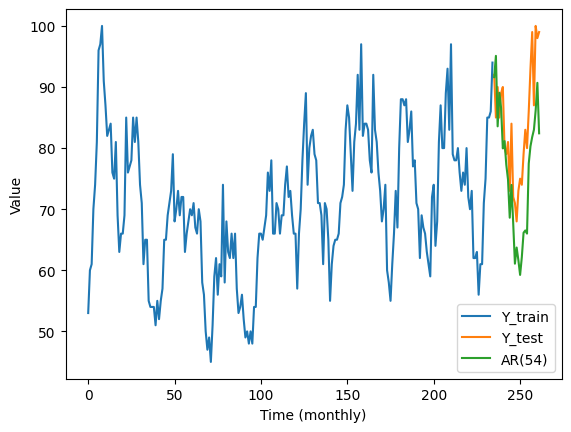
\includegraphics[width=0.7\textwidth]{./static/completed_image.png}
    \caption{ワイドパンツ検索量の時系列データと予測結果}
    \label{fig:prediction_result}
\end{figure}

\section{実施感想}

本課題を通じて,時系列解析の理論と実践の両面について深く学ぶことができた。

\textbf{工夫点}として,当初はAR(12)モデル単体での予測を行っていたが,複数のAR次数(12, 24, 36, 54)を系統的に比較することで最適なモデル選択を試みた点が挙げられる。また,Google Trendsという実世界のデータを用いることで,理論だけでは理解できない現実的な課題に直面することができた。データの前処理や可視化についても,pandas とmatplotlibを活用して効率的に実装できた。

\textbf{難しかった点}は,主に以下の3つである。第一に,ARモデルの適切な次数選択が挙げられる。元のデータの性質を考慮して次数を選択する必要があった。第二に,ファッショントレンドのような急激な変化を持つデータでは,線形モデルである ARでは限界があることを実感した。第三に,statsmodelsライブラリの使用方法の習得に時間を要した。

\textbf{学び}として最も印象的だったのは,時系列予測の難しさである。特に,過去のパターンから未来を予測するというARモデルの基本的な仮定が,急激な社会変化やトレンドの転換点では通用しないことを体験できた。また,複数のモデルを比較することの重要性や,予測精度を定量的に評価する手法(RMSE,MAE)の実用性についても理解を深めることができた。この経験は,実際のビジネス場面での予測精度の限界を認識し,不確実性を考慮した意思決定の重要性を学ぶ貴重な機会となった。

\section{AR次数比較実験}

\subsection{実験設定}
ARモデルの次数 $r$ がモデル性能に与える影響を検証するため,以下の4つの次数で比較実験を実施した:
\begin{itemize}
\item AR(12):四半期季節性(週次データで約3ヶ月分)を考慮
\item AR(24):より長期の依存関係を考慮(約6ヶ月分)
\item AR(36):長期依存関係の強化(約9ヶ月分)
\item AR(54):最長期の依存関係(約1年分)
\end{itemize}

\subsection{予測精度の比較}
各ARモデルの予測精度を RMSE(Root Mean Square Error)および MAE(Mean Absolute Error)で評価した結果は以下の通りである:

\begin{center}
\begin{tabular}{|c|c|c|}
\hline
AR次数 & RMSE & MAE \\
\hline
AR(12) & 13.11 & 9.70 \\
AR(24) & 11.68 & 9.60 \\
AR(36) & 10.81 & 8.85 \\
AR(54) & 10.15 & 8.81 \\
\hline
\end{tabular}
\end{center}

\begin{figure}[htbp]
    \centering
    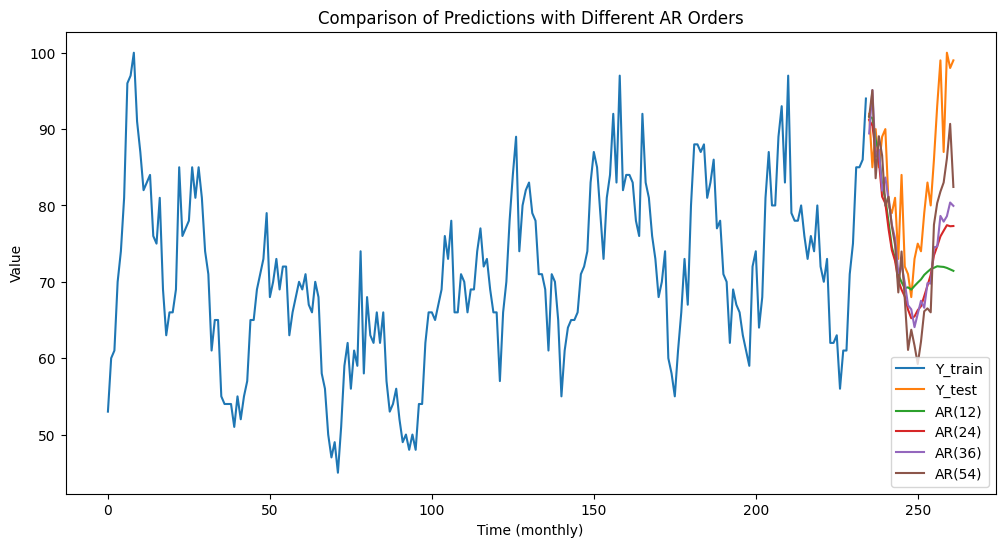
\includegraphics[width=0.7\textwidth]{./static/compare_images.png}
    \caption{異なるAR次数による予測結果の比較}
    \label{fig:ar_comparison}
\end{figure}

\begin{figure}[htbp]
    \centering
    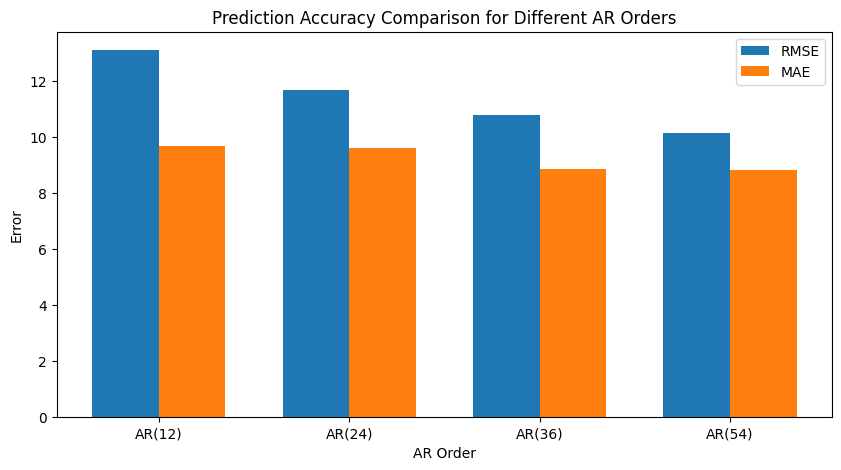
\includegraphics[width=0.7\textwidth]{./static/compare_difference.png}
    \caption{AR次数別の予測精度比較(RMSE・MAE)}
    \label{fig:accuracy_comparison}
\end{figure}

\subsection{結果分析と考察}
実験結果から以下の知見が得られた:

\subsubsection{次数増加による精度向上}
ARの次数を12から54に増加させることで,RMSE は 13.11 から 10.15 へ(約22.5\%改善),MAE は 9.70 から 8.81 へ(約9.2\%改善)となり,明確な予測精度の向上が確認された。

\subsubsection{改善効果の漸減傾向}
次数増加に伴う精度改善は漸減傾向を示しており,AR(36)からAR(54)への改善幅はAR(12)からAR(24)への改善幅よりも小さくなっている。これは,過度に長期の依存関係を考慮することの限界効果を示している。

\subsubsection{計算複雑性とのトレードオフ}
次数の増加は予測精度向上をもたらす一方で,パラメータ数の増加により計算複雑性も増大する。今回は問題なかったが,実用的な観点では,精度向上と計算コストのバランスを考慮する必要がある。

\subsection{最適次数の選択}
本実験においては,\textbf{AR(54)が最も優れた予測性能}を示した。その根拠は以下の通りである:

\begin{enumerate}
\item \textbf{予測精度}:全ての評価指標(RMSE, MAE)において最良の値を記録
\item \textbf{データ特性への適合}:週次データにおいて約1年分の履歴を考慮することで,年次周期性を効果的に捉えることが可能
\item \textbf{安定性}:学習データサイズ(235点)に対して適切なパラメータ数(54個)であり,過学習のリスクが比較的低い
\end{enumerate}

ただし,実際の運用では確保可能な計算資源に応じて,AR(36)も実用的な選択肢となり得る。

\section{結論}

本研究では,自己回帰モデル(AR)の理論的理解と実践的応用を通じて,時系列解析の基礎的手法を習得した。Google Trendsの「ワイドパンツ」検索量データを用いた実験により,以下の重要な知見を得ることができた:

\begin{enumerate}
\item ARモデルは周期的パターンを持つ時系列データに対して有効な予測手法である
\item 適切な次数選択により予測精度の大幅な改善が可能である(本実験では AR(54) が最適)
\item ファッショントレンドのような急激な変化を含むデータでは,線形モデルの限界が存在する
\item 実世界のデータ分析では,理論的知識と実践的な試行錯誤の両方が重要である
\end{enumerate}

\end{document}
